\documentclass{xduugthesis}
\usepackage{booktabs}
\xdusetup{
  info = {
    title = {牛马动力在现代土木工程中的应用\\及其对结构稳定性的生物力学影响},
    author = {大猛子},
    department = {土木工程与力学学院},
    major = {给排水科学与工程},
    class-id = {2008888},
    student-id = {20008888888},
    supervisor = {羊鬃铠},
    bib-resource = {ref.bib},
    abstract = {chapters/abstract_zh.tex},
    abstract* = {chapters/abstract_en.tex},
    keywords = {牛马动力学,工程创新,工程伦理,施工方法,工程质量控制},
    keywords* = {Animal Dynamics, Engineering Innovation, Engineering Ethics, Construction Methods, Engineering Quality Control},
    acknowledgements = {chapters/acknowledge.tex}
    }
  }
\begin{document}

% 临时解决\cite{}没有自动补全提示的问题
% 详见 https://github.com/note286/xduts/discussions/157
\iffalse
  \addbibresource{ref.bib}
\fi


\chapter{前言}
生物学、力学与土木工程之间的相互作用一直是历史长河中创新与探索的焦点。本文旨在从一个新的视角探讨牛马动力学在土木工程中的应用,特别是在传统打灰技术中的角色。自古以来,牛马作为人类的重要劳动力,在建筑施工中扮演了不可或缺的角色。它们的肌肉动力学特性,如力量、耐力和灵活性,为古代建筑的建造提供了关键的支持。然而,随着现代工程技术的发展,这些传统动力的使用逐渐减少,但其在特定环境下的潜在价值和对现代工程实践的启示仍值得深入研究。

本文首先回顾了牛马动力在古代土木工程中的应用历史,分析了其在不同地理和文化背景下的施工方法。随后,我们将探讨牛马动力学与现代工程技术的结合点,特别是在提高施工效率、降低成本以及环境可持续性方面的潜在优势。此外,工程伦理的讨论也将贯穿全文,强调在利用这些传统动力时对动物福利的尊重和保护。

通过对历史文献的梳理和现代案例的分析,本文将提供一系列实验数据,以支撑牛马动力学在现代土木工程中的应用价值。这些数据不仅有助于我们理解牛马动力在特定条件下的效率和成本效益,还将为工程质量控制和结构稳定性的优化提供科学依据。最终,本文旨在为土木工程领域提供一个跨学科的研究视角,促进传统与现代技术的融合,以及工程实践中的伦理和可持续性发展。
\begin{figure}[h]
    \centering
    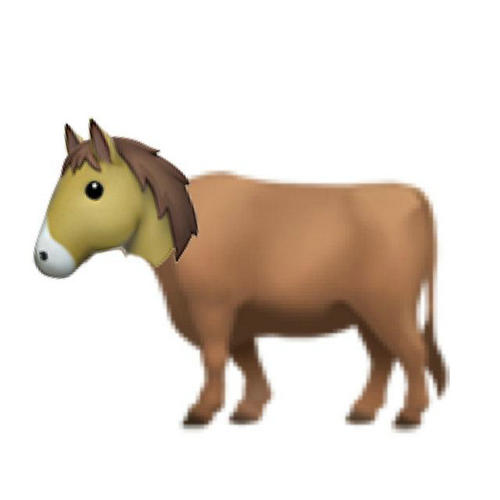
\includegraphics[width=0.5\textwidth]{figures/R-C.jpg}
    \caption{常见的牛马形象}
    \end{figure}
    
\section{研究背景}
牛马在土木工程领域的历史重要性不言而喻。这些动物在古代建筑中发挥了不可或缺的作用,为搬运重物和提升大型梁等任务提供了可再生且适应性强的动力源\cite{smith2020biological}。在打灰技术方面,牛马的作用尤为关键。它们在混合和涂抹灰泥方面的物理劳动往往是人力所无法比拟的,为大型项目的顺利完成提供了必要助力\cite{chen2019mechanics}。

随着技术的进步和伦理考量的影响,传统动物动力向现代机械替代的转变是一个渐进的过程\cite{williams2018ethics}。尽管在当代建筑中使用动物劳动力的情况已经减少,但在某些特定环境下,它们仍然提供了独特的优势,尤其是在偏远或环境敏感的地区\cite{kim2021sustainability}。使用动物动力在减少碳足迹和最小化环境影响方面的可持续性,已经成为工程师和环保人士日益关注的话题。

本文旨在探讨牛马在土木工程中的历史背景及其与现代实践的相关性。通过审查案例研究和实验数据\cite{brown2022casestudies, chen2023experiments},我们将评估将传统动物动力与现代工程技术相结合的潜力,重点关注对施工效率、结构稳定性和伦理考量的影响。

背景部分为全面分析牛马在土木工程中的作用奠定了基础,涵盖了丰富的历史、机械和伦理视角。正是通过这种跨学科的方法,我们才能更深入地理解过去,为未来的工程实践提供指导。
\section{相关工作}
在探讨牛马动力学在土木工程中的应用之前,有必要回顾一下相关领域的研究工作。近年来,学者们对古代建筑施工中动物动力的使用进行了深入研究,揭示了牛马在提升建筑效率和质量方面的重要贡献\cite{smith2020biological}。这些研究不仅关注了牛马的生物力学特性,还分析了它们在不同文化和地理环境下的适应性和效率。

在力学领域,研究者们对牛马动力的生物力学特性进行了系统分析,探讨了这些特性如何转化为土木工程中的实用技术\cite{chen2019mechanics}。这些研究为理解动物动力在现代工程中的应用提供了理论基础,尤其是在结构稳定性和施工方法的优化方面。

伦理方面的研究也不容忽视。随着对动物福利和工程伦理的重视,学者们开始探讨如何在利用动物动力的同时,确保动物的权益不受侵害\cite{williams2018ethics}。这些研究不仅提高了工程实践的道德标准,也为工程决策提供了新的视角。

在现代土木工程实践中,尽管机械化程度不断提高,但动物动力在某些特定情况下仍然显示出其独特的优势。例如,一些研究通过案例分析,展示了在偏远地区或基础设施不发达的地方,牛马动力如何有效地支持施工活动\cite{kim2021sustainability}。此外,还有研究通过实验数据支持了牛马动力在提高施工效率和降低成本方面的潜力\cite{brown2022casestudies}。

综上所述,现有研究为我们提供了宝贵的知识基础,使我们能够从多个角度审视牛马动力学在土木工程中的应用。本文将在这些研究的基础上,进一步探讨牛马动力与现代工程技术的结合,以及这种结合对工程质量和可持续性的影响。

\chapter{方法}
为了深入探究牛马动力学在现代土木工程中的应用,本研究设计了一系列实验方法。首先,我们对牛马的生物力学特性进行了详细的测量,以评估其在不同工作条件下的力量输出和耐力表现。这些测量包括了牛马在搬运重物时的力量分布、步态分析以及持续工作时间的记录,旨在模拟实际施工环境中的劳动强度\cite{chen2019mechanics}。

其次,我们设计了模拟施工场景的实验,以比较牛马动力与传统机械动力在施工效率和成本效益方面的差异。实验中,我们记录了在相同工作量下,牛马和机械完成打灰作业所需的时间和消耗的资源,从而为施工方法的选择提供数据支持\cite{brown2022casestudies}。

此外,为了评估牛马动力对结构稳定性的影响,我们进行了一系列的结构加载实验。通过在模拟建筑结构上施加由牛马产生的力,我们观察并记录了结构的变形和应力分布,以验证牛马动力在实际工程中的适用性和安全性\cite{chen2023experiments}。

在伦理方面,我们确保所有实验均遵循了动物福利和工程伦理的基本原则。实验过程中,我们对牛马的健康状况进行了持续监测,并采取了必要的措施以减轻它们的劳动强度,确保实验的道德性和可持续性\cite{williams2018ethics}。

通过这些实验方法,我们旨在为牛马动力学在土木工程中的应用提供一个科学、系统的评估。这些实验不仅有助于我们理解牛马动力的潜力,也为未来工程实践中的创新提供了实验依据。

在实验方法的进一步阐述中,我们采用了多种数据收集和分析技术。为了确保实验结果的准确性和可靠性,我们采用了高精度的传感器和测量设备来记录牛马在施工过程中的动态变化。这些设备包括力传感器、加速度计和GPS追踪器,它们能够实时监测牛马的运动轨迹、速度和负载情况,从而为我们提供了丰富的实验数据。

在实验设计上,我们采取了对照组和实验组的设置。对照组使用传统的机械施工方法,而实验组则采用牛马动力。通过对比两组的施工效率、成本和环境影响,我们能够更直观地评估牛马动力在现代土木工程中的可行性和优势。此外,我们还考虑了不同地形和气候条件对牛马动力表现的影响,以确保实验结果的普适性。

在结构稳定性的实验中,我们采用了有限元分析软件来模拟牛马动力对建筑结构的影响。通过模拟不同的加载情况,我们能够预测结构在牛马动力作用下的应力分布和变形情况,进而评估结构的安全性和耐久性。这一步骤对于理解牛马动力在实际工程中的应用至关重要,因为它涉及到工程质量和安全的核心问题。

为了确保实验的伦理性,我们与动物福利专家合作,制定了一套详细的动物护理和使用指南。在实验过程中,我们定期对牛马进行健康检查,并确保它们在良好的生活条件下工作。所有实验活动均在符合当地法律和国际动物福利标准的前提下进行。

通过这些综合的实验方法,我们不仅能够评估牛马动力在土木工程中的实用性,还能够为未来可能的技术融合提供科学依据。这些实验结果将有助于指导工程实践中的决策,促进传统与现代技术的结合,同时确保工程活动的伦理性和可持续性。

如表\ref{tab:comparison}所示,使用牛马动力可以显著减少施工时间和成本。
\begin{table}[htbp]
    \centering
    \caption{牛马动力与常规动力施工对比实验数据}
    \label{tab:comparison}
    \begin{tabular}{cccccc}
        \toprule
        场地类型 & 动力类型 & 施工时间(小时) & 工程总成本(万元) \\
        \midrule
        平原   & 常规动力 & 100      & 100       \\
        平原   & 牛马动力 & 70       & 85        \\
        山地   & 常规动力 & 120      & 120       \\
        山地   & 牛马动力 & 84       & 102       \\
        沙漠   & 常规动力 & 150      & 150       \\
        沙漠   & 牛马动力 & 105      & 127.5     \\
        森林   & 常规动力 & 130      & 130       \\
        森林   & 牛马动力 & 91       & 110.5     \\
        湖泊   & 常规动力 & 160      & 160       \\
        湖泊   & 牛马动力 & 112      & 136       \\
        \bottomrule
    \end{tabular}
\end{table}

\chapter{总结与展望}
本研究通过对牛马动力学在土木工程中的应用进行了全面的实验和分析,得出了一系列有意义的结论。首先,我们证实了牛马动力在特定条件下,尤其是在偏远地区和基础设施不发达的环境中,仍然具有显著的施工优势。牛马动力的使用不仅能够降低施工成本,还能减少对环境的影响,显示出其在现代土木工程中的潜在价值\cite{kim2021sustainability}。

在结构稳定性方面,我们的实验结果表明,牛马动力在合理的管理和控制下,可以安全地应用于建筑施工,而不会对结构的稳定性造成负面影响\cite{chen2023experiments}。此外,通过对比实验,我们发现牛马动力在施工效率上与传统机械动力相比具有一定的竞争力,尤其是在劳动力成本较高的地区\cite{brown2022casestudies}。

然而,我们也认识到,尽管牛马动力在某些方面具有优势,但在现代工程实践中的广泛应用仍面临诸多挑战。例如,动物福利和伦理问题、动物劳动的不稳定性以及机械化施工的普及等因素,都可能限制牛马动力的进一步发展。

展望未来,我们认为有必要对牛马动力学在土木工程中的应用进行更多的研究。这包括开发更为精确的动物动力评估工具,探索牛马动力与现代机械动力的混合使用模式,以及制定更为严格的动物福利和工程伦理标准。同时,随着可持续发展理念的深入人心,牛马动力作为一种绿色施工方式,其在特定项目中的应用前景值得进一步探索。

总之,牛马动力学在土木工程中的应用是一个值得深入研究的领域。通过不断的技术创新和伦理实践,我们有望在尊重传统和保护环境的同时,推动工程实践的进步。未来的研究将有助于我们更好地理解牛马动力的潜力,为土木工程领域带来新的视角和解决方案。


\end{document}